\chapter{Point de vue developpeur}

\section{Documentation}
qsdqsd
\clearpage
\section{Conception}
\subsection{Architecture}
Dans cette partie nous détaillerons l'architecture de notre application, à travers ses différents points d'extensions.
\begin{figure}[!htbp]
  \centering
  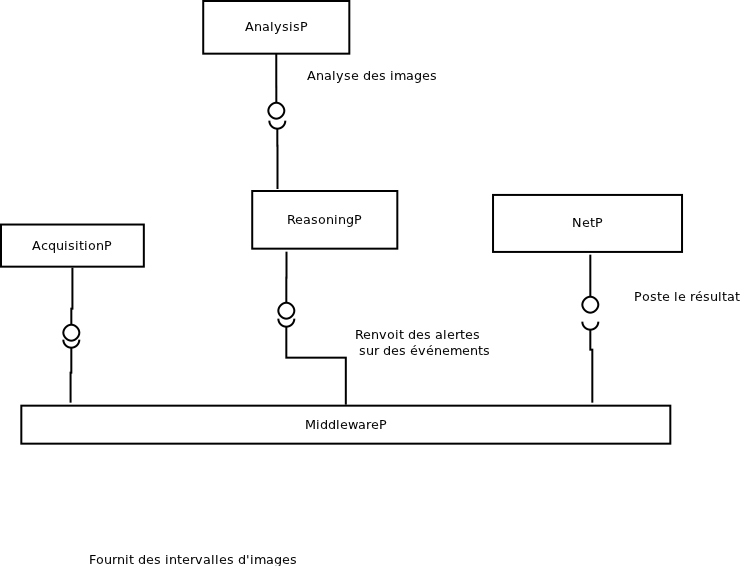
\includegraphics[scale=0.50]{img/archi}
  \caption{Architecture de l'outil}
  \label{fig:archi}
\end{figure}

\subsection{Classes}
dsqdqs
\paragraph{Architecture}
qsdqs
\paragraph{Acquisition}
dqsdsq
\paragraph{Reasoning}
sdqsd
\paragraph{NetP}
Le  NetP est dédié à poster des informations sur un  réseau social ou un blog. Un contributeur de ce point d'extension doit être en mesure de proposer une solution pour chaque action que recquière Middleware. Ces actions sont données dans l'interface \verb+IIformation+ suivante :
\begin{figure}[!htbp]
  \centering
  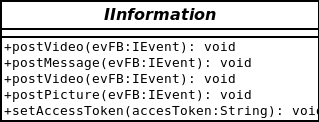
\includegraphics[scale=0.50]{img/iinterface}
  \caption{Interface pour NetP}
  \label{fig:IInterface}
\end{figure}

Le contributeur que nous avons implémenté propose d'utiliser le réseau social Facebook et utilise la librairie suivante \cite{restFB}.


\section{Robustesse}
sqdqs
\section{Qualité du code}
dqsdqs
\section{Facilité de mise en oeuvre des extension}
